\section{Method}\label{sec:method}
% --------------------------------
Here, we introduce \emph{Okapi}, a simple, efficient, and general (in the sense that it is
applicable to any task \emph{or} modality) method for robust semi-supervised learning based on
online statistical matching. 
%
Our method belongs to the broad family of consistency-based methods, characterised by methods such
as FixMatch \citep{sohn2020fixmatch}, where the idea is to enforce similarity between a model's
outputs for two views of an unlabelled image. 
%
These semi-supervised approaches based on minimising the discrepancy between two views of a given
sample are closely related with self-supervised methods based on instance discrimination
\citep{chen2020simple} and self-distillation
\citep{baevski2022data2vec,caron2021emerging,grill2020bootstrap}.
%
Many of the methods within this family, however, are limited in applicability due to their
dependence on modality-specific transformations and only recently has research into
self-supervision sought to redress this problem with modality-agnostic alternatives such as MixUp
\citep{verma2021towards}, masking \citep{baevski2022data2vec}, and nearest-neighbours
\citep{dwibedi2021little, koohpayegani2021mean, van2021revisiting}.
%
Approaches such as FixMatch, AlphaMatch \citep{gong2021alphamatch} and CSSL
\citep{lienen2021credal} that enforce consistency between the \emph{predictive} distributions
suffer further from not being directly generalisable to tasks other than classification.
%
Okapi addresses both of these aforementioned issues through 1) the use of a statistical matching
procedure -- that we call \CNN{} and detail in \S\ref{subsec:matching} -- to generate multiple
views for a given sample; 2) enforcing consistency between encodings rather than between predictive
distributions.

We show that models trained to maximise the similarity between the encoding of a given sample and
those of its \CNN{}-generated match are significantly more robust to real-world distribution shifts
than the baseline methods, while  having the advantage of being both computationally efficient and
agnostic to the modality and task in question.
%
Qualitatively speaking, we see that matches produced with the final model are related in
semantically-meaningful ways. 
%
Furthermore, since the only constraint is that samples be from different domains, the method is
applicable whether information about the domain is coarse or fine-grained.
%

In the following subsections, we begin by giving a general formulation of our proposed
semi-supervised loss employing a generic cross-domain $k$-NN algorithm. 
%
We then explain how we can replace this algorithm with \CNN{} in order to mitigate the risk of
poorly-matched samples, and how the loss may be computed in an online fashion to give our complete
algorithm.

\subsection{Enforcing consistency between cross-domain pairs}
%
We consider our predictor as being composed of an encoder (or \emph{backbone}) network, $f_\theta:
\gX \to \R^d$, generating intermediary outputs (features) $z \triangleq
f_\theta(x)$, and a prediction head, $g_\phi$, such that the prediction for sample $x$ is given by
$\hat{y} \triangleq g_\phi \circ f_\theta(x)$.
%
We similarly consider the aggregate loss $\gL$ as having a two-part decomposition given by
%
\begin{equation} \gL \triangleq \gL_{\mr{sup}} + \lambda \, \gL_{\mr{unsup}},
\end{equation}
%
where $\gL_\mr{sup}$ is the supervised component measuring the discrepancy (as computed, for
example, by the MSE loss) between $\hat{y}$ and the ground-truth label $y$, $\gL_{\mr{unsup}}$
is the unsupervised component based on some kind of pretext task, such as cross-view consistency,
and $\lambda$ is a positive pre-factor determining the trade-off between the two components.
%
For our method, we do not assume any particular form for  $\gL_{\mr{sup}}$ and focus solely on
$\gL_\mr{unsup}$.
%

Given a pair of datasets $\gD_l$ and  $\gD_u$, sourced from the labelled domain $\gS_l$,
and unlabelled domain $\gS_u$ respectively, along with their union $\gD \triangleq \gD_l
\cup \gD_u$ our goal is to train a predictor that is robust (invariant) to changes in domain,
including those unseen during training.
%
To do this, we propose to regularise $z \triangleq f_\theta(x)$ to be smooth (consistent) within
local, cross-domain neighbourhoods.
%
At a high-level, for any given \emph{query} sample $x_q$ sourced from domain $s_q$, we compute
$\gL_{\mr{unsup}}$ as the mean distance between its encoding $z_q \triangleq f_\theta(x_q)$ and
that of its $k$-nearest neighbours, $V_k(z_q)$ with the constraint that $\{ s_q \} \cap \mbf{s}_n =
\emptyset$, where $\mbf{s}_n$ is the set of domain-labels associated with $V_k(z_q)$.
%
The general form of this loss for a given sample can then be written as
\begin{align}
    V_k(z_q) &\triangleq \mr{NN}(z_q, \{ f_\theta(x)\;|\; (x, s) \in \gD, s \neq s_q \}, k),
    \label{cgnn} \\
    \gL_{\mr{unsup}} &\triangleq \frac{1}{k} \sum_{z_n \in V_k(z_q)} d(z_q, z_n)
\end{align}
%
where $d: \R^d \times \R^d \to \R$ is some distance function.
%
Here, we follow \citet{grill2020bootstrap} and define $d$ to be the squared Euclidean distance
between normalised encodings for our experiments.
%
Allowing the $\mr{NN}$ algorithm to select pairs in an unconstrained manner, given the pool of
queries and keys, however, can lead to poorly-matched pairs that are detrimental to the
optimisation process.
%
To address this, we replace the standard $\mr{NN}$ algorithm with a propensity-score-based variant,
inspired by the statistical matching framework \citep{rosenbaum1983central}.
%
\subsection{Cross-domain matching}\label{subsec:matching}
%
For the matching component of our algorithm, we propose to use a variant of $k$-NN which, in
addition to incorporating the above cross-domain constraint, filters the queries and keys that
represent probable outliers, according to their learned propensity scores.
%
The initial stage of filtering employs a fixed caliper, where samples with propensity scores
surpassing a fixed confidence threshold are removed; this is followed by a second stage of
filtering wherein any two samples (from different domains) can only be matched if the Euclidean
distance between their respective propensity scores is below a pre-defined threshold (std-caliper).
%
See Fig~\ref{fig:calipernn_pipeline} for a pictorial representation of these steps and
Appendix~\ref{appx:pseudocode} for reference pseudocode.

\begin{figure}[tbp]
  \centering
  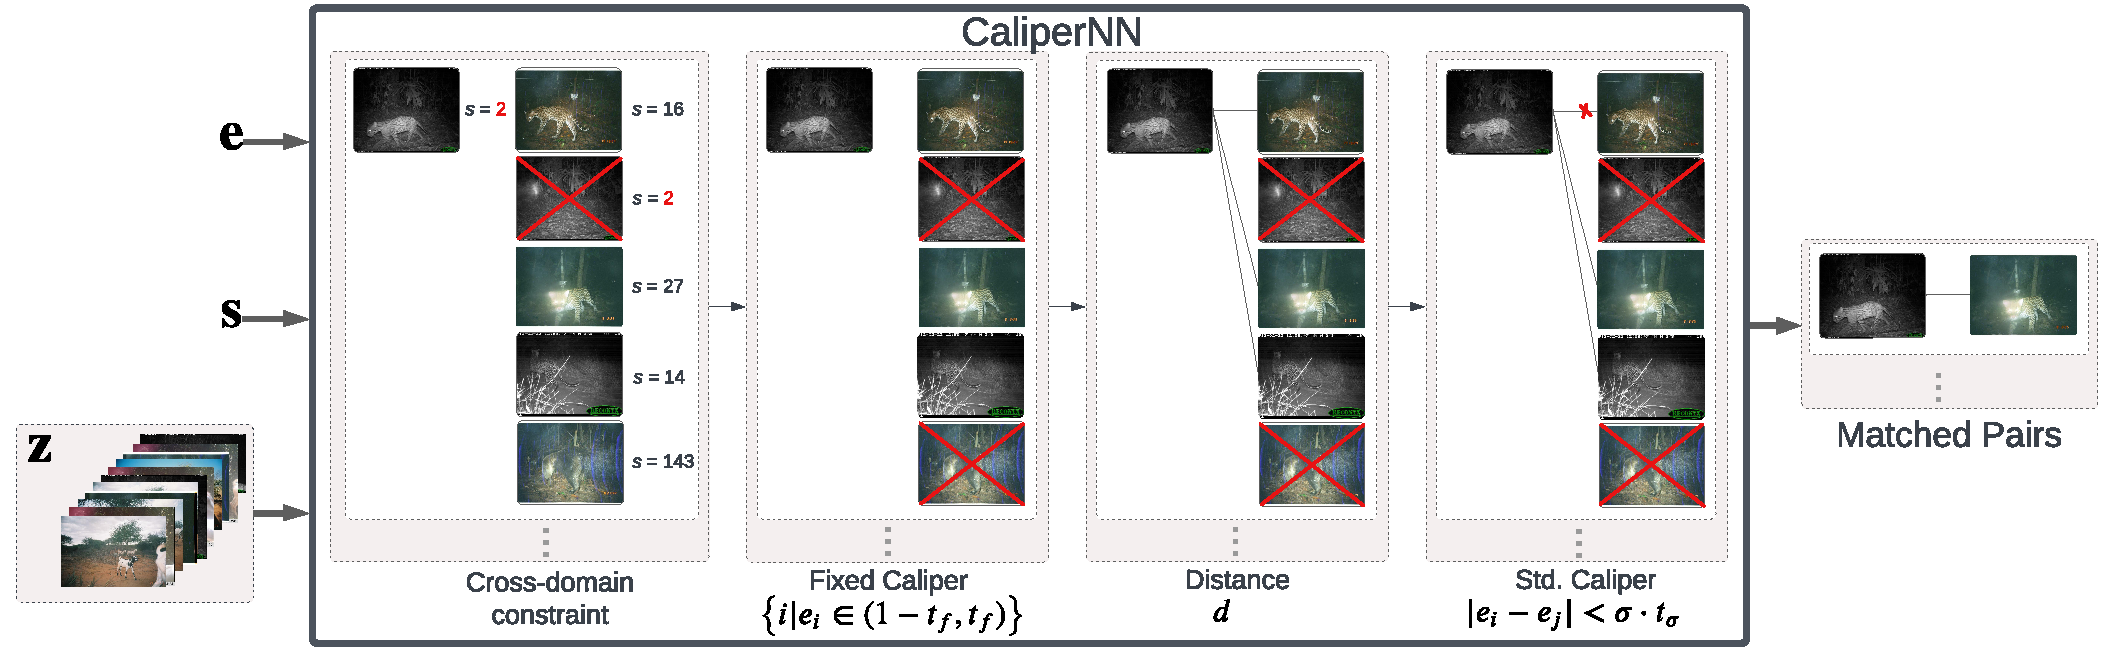
\includegraphics[width=1.\textwidth]{figures/CaliperNN_PS_pipeline.pdf}
  \caption{
    %
    Illustration of our proposed statistical matching algorithm, \CNN{}. 
    %
    Given the encoding, $\mbf{z}$, of some anchor (query) image, the corresponding domain label
    $s$, and propensity score $e$, \CNN{} yields the closest samples, according to distance $d$,
    subject to the constraint that those samples belong to a different domain to the anchor
    (cross-domain constraint), as well as the constraints imposed by the two calipers.
    %
    Red crosses denote exclusion of the keys from the pool of candidate-matches, such that the
    \(k\)-closest (\(k\) being \(1\) here for simplicity's sake) unmarked samples become the
    outputs of the matching algorithm.
    %
    The fixed caliper filters samples based on a fixed-value thresholding of the propensity scores,
    such that samples that have sufficiently (adjudged by the threshold, \(t_{f}\)) extreme
    propensity scores, which is to say are overly-characteristic of their respective domains, are
    removed from the pool of candidate-matches. 
    %
    In the corresponding sub-figure, the set of samples at this stage is singular, consisting
    of only the bottom-most image (key).
    %
    The standard-deviation (std.) caliper, on the other hand, filters based on an adaptive
    threshold -- modulated by a predefined pre-factor \(t_{\sigma}\) -- computed from the standard
    deviation of the propensity scores. 
    %
    In the corresponding sub-figure, exclusion by the std. caliper is denoted with a red
    cross over the top-most edge, leaving only two candidates keys, the top-most of which is
    implied to be closest by its selection in the final step.
  %
    For more details pertaining the calipers, their provenance, and their rationale, vide \S2.1 of
    \citet{RomInsShaQua22}.
    % CORRECTED: could add a little more detail on the steps here
}
  \label{fig:calipernn_pipeline}
\end{figure}

%
The propensity score, $e$, for a given sample $x$ is estimated as $p(s|z)$ using a linear
classifier $f_\theta$, $h_\psi: \R^d \to \bigtriangleup^{|\gS|}$ where $\bigtriangleup^{|\gS|}$ is
the probability simplex over possible domain labels, $\gS$. $h_\psi^d$ is trained via maximum
(weighted) likelihood to predict the domain label of a given sample for all samples within the
aggregate dataset $\gD$, or (typically) a subset of it, encoded by $f_\theta$.
%
Since we apply both calipers to the learned propensity score, the shape of this distribution can
have a significant effect on the outcome of matching.
%
Accordingly, we apply temperature-scaling, with scalar $\tau \in \R^+_\ast$, to the logits of
$h_\psi$ (where $\bigtriangleup^{|\gS|}$ is induced by the softmax function) to modulate the
resulting propensity-score distribution.
%
We denote the set of associated parameters (\{ $t_{f}, t_{\sigma}, \tau \}$, as the threshold for
the fixed-caliper, the threshold for the std-caliper, and the temperature, respectively) as $\xi$
and discuss in Appendix~\ref{appx:implementation} how one can determine suitable values for these
in practice.

For convenience we define the set of all encodings, given by $f_\theta$, as $\mbf{z} \triangleq \{
f_\theta (x)\, |\, x \in \gD \}$, the set of all associated propensity scores as $\mbf{e}
\triangleq \{ h_\psi (x) \, | \, z \in \mbf{z} \}$, and the set of associated domain labels as
$\mbf{s}$.
%
In the offline case, the matches for $\gD$ are then computed as
%
\begin{equation}
  \mr{MatchedSamples} \triangleq \{ (z,  \mr{\CNN{}}_\xi(z, \mbf{z}, \mbf{e}, s, k)) \, | \, z \in
    \mbf{z}, s \in \mbf{s} \},
\end{equation}
%
with \CNN{} returning the set of $k$-nearest neighbours according to $d$, subject to the
aforementioned cross-domain and caliper-based constraints. We allow for the fact that there may be
no valid matches for some samples due to these constraints; in such cases we have $\emptyset$ as
the second element of their tuples, indicating that $\gL_{\mr{unsup}}$ should be set to $0$.
%
\subsection{Scaling up with Online Learning}\label{subsec:ol}
%
Re-encoding the dataset following each update of the feature-extractor, in order to recompute
$\mr{MatchedSamples}$, is prohibitively expensive, with cost scaling linearly with $N \triangleq
N_l + N_u$.
%
Moreover, \CNN{} requires explicit computation of the pairwise distance matrices, which can be
prohibitive memory-wise for large values of $N$.
%
We address these problems using a fixed-size memory bank, $\gM^{\NM}_z$ storing only the last $\NM$
(where $\NM \ll N$) encodings from a slow-moving momentum encoder \citep{grill2020bootstrap,
he2020momentum}, $\textcolor{tecol}{f_{\theta^\prime}}$, which we refer to as the
\textcolor{tecol}{\emph{target}} encoder, in line with \citet{grill2020bootstrap}, and accordingly
refer to $\textcolor{oecol}{f_\theta}$ as the \textcolor{oecol}{\emph{online}} encoder.
%
Unlike \citet{grill2020bootstrap}, however, we make use of neither a projector nor a predictor head
(in the case of the target encoder) in order to compute the inputs to the consistency loss and
simply use the output of the backbone as is -- this is possible in our setting due to
$\gL_\mr{sup}$ preventing representational collapse.
%
More specifically, the target encoder's parameters, $\textcolor{tecol}{\theta^\prime}$, are computed as a moving
average of the online encoder's, $\textcolor{oecol}{\theta}$, with decay rate $\zeta \in (0, 1)$, per the recurrence
relation
%
\begin{equation}
  \textcolor{tecol}{\theta^\prime_t} = \zeta \textcolor{tecol}{\theta^\prime_{t - 1}} + (1 - \zeta)
  \textcolor{oecol}{\theta_t},
\end{equation}
%
As the associated domain labels are also needed both for matching and to compute the loss for the
propensity scorer, we also store the labels associated with $\gM^{\NM}_z$ in a companion memory bank
$\gM^{\NM}_s$. 
%
We initialise $\gM^{\NM}_z$ and $\gM^{\NM}_s$ to $\emptyset$, resulting in
fewer than $\NM$ samples being used during the initial stages of training when the memory banks are
yet to be populated.
%

Each iteration of training, we sample a batch of size $B$ from $\gD$ consisting of inputs $\mbf{x}$
and $\mbf{s}$.
%
During the matching phase, the inputs are passed through the \emph{target} encoder to obtain
$\mathbf{z}_q^\prime \triangleq \{ \textcolor{tecol}{f_{\theta^\prime} } (x) | x \in \mbf{x}\}$,
serving as the queries for \CNN{}.
%
We also experiment with a simpler variant where the \emph{online} encoder is instead used for this
query-generation step, such that we instead have $\mathbf{z}_q^\prime \triangleq
\{\textcolor{oecol}{f_{\theta}}(x) | x \in \mbf{x}\}$, and find this can work equally well if
$\zeta$ is sufficiently high.
%
The keys are then formed by combining the current queries with the past queries contained in the
memory bank: $\mbf{z}_k\triangleq \mathbf{z}_q^\prime \cup \gM^{\NM}_z$.
%
The domain labels associated with $\mbf{z}_k$ are likewise formed by concatenating the domain
labels in the current batch with those stored in $\gM^{\NM}_s$: $\mbf{s}_k \triangleq \mbf{s}_q \cup
\gM^{\NM}_s$.
%
Once the matches for the current samples have been computed, the oldest $B$ samples in $M^{\NM}_z$
and $M^{\NM}_s$ are overwritten with $\mathbf{z}_k$ and $\mathbf{s}_k$, respectively.
%
The consistency loss is then enforced between each query $\mathbf{z}_q \triangleq \{
  \textcolor{oecol}{f_{\theta}}(x) |
x \in \mbf{x}\} $, according to the differentiable \emph{online} encoder, and each of its matches,
$V_k(z_q^\prime) \triangleq \mr{\CNN{}}_\xi(z_q, \mbf{z}_k, h_\psi(\mbf{z}_k), \mbf{s}_k)$ providing
that $V_k(z_q^\prime) \neq \emptyset$ (that is, under the condition that the estimated propensity
score for $z_q^\prime$ does not violate the caliper(s) and there are at least $k$ valid matches
whose estimated propensity scores also do not), with the loss simply $0$ otherwise.
%
Since $\textcolor{tecol}{ f_{\theta^\prime} }$ is frozen, $\mbf{z}_k$ carries an implicit
stop-gradient and gradients are computed only \wrt{} $\textcolor{oecol}{ \theta}$.
%
These steps are illustrated pictorially in Fig~\ref{fig:okapi-pipeline} and as pseudocode in
Appendix~\ref{appx:pseudocode}.

Similarly, rather than solving for the optimal parameters, $\psi^\star$ for the propensity scorer
given the current values of $\mbf{z}_k$, which is infeasible for the large values of $\NM$ needed
to well-approximate the full dataset, we resort to a biased estimate of $\psi^\star$.
%
Namely, we train $h_\psi$ in an online fashion to minimise the per-batch loss 
%
\begin{equation}
\gL_\mr{ps} = \frac{1}{|\mbf{z}_k|} \sum_{ z \in \mbf{z}_k, s \in \mbf{s}_k } w_{\mbf{s}_k}(s) \gH(h_{\psi}(z), s), 
\end{equation}
%
where $\gH$ is the standard cross-entropy loss between the predictive distribution and the
(degenerate) ground-truth distribution, given by the one-hot encoded domain labels, and
$w_{\mbf{s}_k}: \gS \to \R^+_*$ is a function assigning to each $s$ an importance weight
\citep{shimodaira2000improving} based on the inverse of its frequency in $\mbf{s}_k$ to counteract
label imbalance.
%
In the special case in which the $\gD_l$ and $\gD_u$ are known to have disjoint support over $S$
(that is, $\gS_l \cap \gS_u = \varnothing$), we can substitute their domain labels with $1$ and
$0$, respectively (such that we have $\gD_l \triangleq \{ x_i, y_i, 1 \}_{i=1}^{N_l}$ and $\gD_u
\triangleq \{x_i, 0 \}_{i=1}^{N_u}$), thus reducing the propensity scorer and \CNN{} to their
binary
forms. 
%
\begin{figure}[ht]
  \centering
  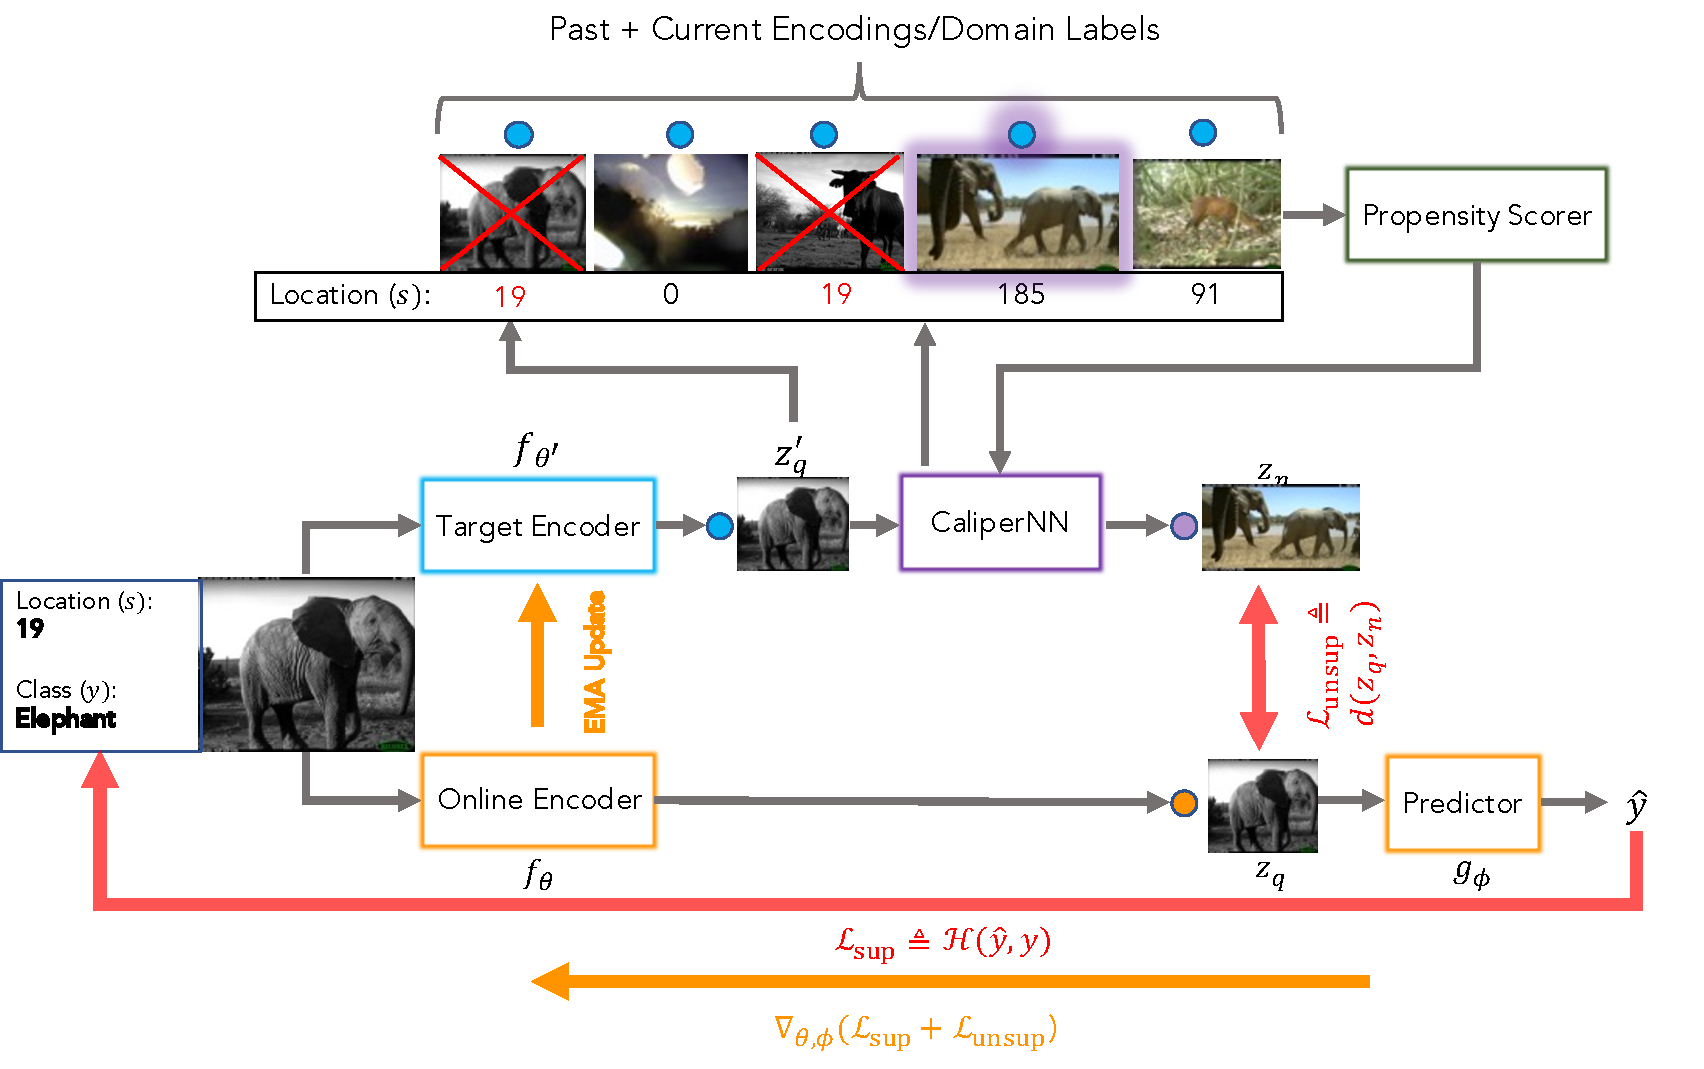
\includegraphics[width=0.9\textwidth]{figures/ol_pipe_new_new.pdf}
  \caption{
    %
  Overview of Okapi's online-learning pipeline based using the iWildCam dataset for the sake of
  illustration.
  %
  For simplicity, we limit $k$ to 1 so that the output of matching is a single vector rather than a
  set of vectors; for the same reason we illustrate the process for only a single sample taken from
  the labelled data set $\gD_l$, annotated with both domain ($s$; in this case, \emph{camera
  location}) and class ($y$) information.
  %
  Inspired by recent advances in self-supervised learning, we maintain a copy (the target encoder)
  of the online encoder, $f_\theta$, whose parameters, $\theta^\prime$, are an exponential moving
  average (EMA) of $\theta$. 
  %
  This EMA update is performed at the beginning of each training set at a rate governed by the
  decay coefficient, $\zeta$. 
  %
  For a given sample, we first compute its embedding using the target encoder to produce the query
  vector, $z_q^\prime$, and by the online encoder to produce $z_q$, which will serve as the
  'anchor' in the consistency loss. 
  %
  This query vector is then used -- alongside the output of the propensity scorer -- by \CNN\ to
  compute its cross-domain nearest neighbour, $z_n$, where the keys are taken to be the current and
  past (stored in the Memory Bank) $N_\gM$ encodings of the data.
  %
  The cross-domain constraint, prohibiting matching of samples belonging to the same domain, is
  denoted through a red colouring of the location identifiers, the nearest sample obeying this
  constraint and the constraints of the calipers with purple highlighting.
  %
  The consistency loss is the distance between $z_q$ and $z_n$, defined by function some distance
  function $d$. 
  %
  Finally, the supervised loss, $\gL_\mr{sup}$ (here instantiated as the standard cross-entropy
  loss, $\gH$), is computed using the output of the predictor acting on $z_q$ and the ground-truth
  given by $y$.
%
  }
  \label{fig:okapi-pipeline}
  %
\end{figure}
%
Knowing whether this condition is satisfied a priori (and thus whether the use of domain labels can
be forgone completely from our pipeline) is not unrealistic: one may, for example know that two
sets of satellite imagery cover two different parts of the world (e.g.\ Africa and Asia) yet not
know the exact co{\"o}rdinates underlying their respective coverage.
